\documentclass[10pt,twocolumn,letterpaper]{article}
\usepackage[margin=0.75in]{geometry}
\usepackage[T1]{fontenc}
\usepackage{newtxtext,newtxmath}
\usepackage{amsmath}
\usepackage{booktabs}
\usepackage{graphicx}
\usepackage{tikz}
\usetikzlibrary{positioning,arrows.meta,fit}
\usepackage[numbers,sort&compress]{natbib}
\usepackage[hidelinks]{hyperref}
\usepackage{xurl}
\usepackage{caption}
\captionsetup{font=small,labelfont=bf}
\setlength{\columnsep}{0.28in}

\title{\textbf{BCI-MCP: Streaming Live EEG Band-Power Metrics to\\AI Assistants over the Model Context Protocol}}
\author{Enkhbold Ganbold\\
\small Independent researcher, Cupertino, California, USA\\
\small \texttt{enkhbold470@gmail.com}}
\date{September 2026}

\begin{document}
\maketitle

\begin{abstract}
Large-language-model (LLM) assistants increasingly call external tools through
the Model Context Protocol (MCP). We describe BCI-MCP, an open-source (MIT)
Python package that exposes live electroencephalography (EEG) from consumer and
research devices to any MCP client. Its central design choice is that the model
never sees raw EEG: a deterministic, documented pipeline (60\,Hz notch,
1--45\,Hz zero-phase band-pass, Welch power spectral density) reduces each 2\,s
window to band powers and six heuristic band-power ratios from the literature,
together with artifact flags, a confidence score, and machine-readable
statements of the pipeline's limitations. We evaluate the released software on
four questions. On synthetic signals with a known generator parameter, all six
metrics track the parameter monotonically (Spearman $|\rho| = 0.996$). On real
EEG from 109 subjects of the PhysioNet EEG Motor Movement/Imagery Dataset, the
unmodified pipeline recovers the eyes-closed alpha increase (Berger effect): the
\emph{calm} metric rises in 105 of 109 subjects (Wilcoxon $p = 3\times10^{-19}$,
rank-biserial $r = 0.99$; within-subject window AUC median 0.87). Injected
artifacts are flagged at fixed amplitude thresholds, but the amplitude-only blink
detector also fires on 40\% of eyes-closed occipital windows, where genuine blinks
are implausible; we report this limitation. A \texttt{get\_brain\_state} tool call over the stdio
transport has a median round-trip latency of 1.3\,ms. The metrics are heuristic
proxies, not validated measures of cognitive state; we discuss what that
implies for LLM-mediated interpretation of neural data.
\end{abstract}

\section{Introduction}

MCP is an open protocol through which an LLM application discovers and calls
\emph{tools}, reads \emph{resources}, and uses \emph{prompts} exposed by
separate server processes~\citep{mcpspec}. It has made it simple to connect an
assistant to a data source. Physiological data is an obvious candidate, and EEG
in particular is now available from inexpensive headsets such as Muse and OpenBCI
boards~\citep{krigolson2017}.

Connecting EEG to an LLM raises a specific risk. A language model asked to
``read'' a brain signal will produce a fluent interpretation whether or not the
data supports one. Handing a model raw samples invites it to invent spectral
analysis; handing it a single ``focus: 0.82'' invites it to treat a heuristic
ratio as a measurement. BCI-MCP is built around the opposite contract: all signal
processing is deterministic and inspectable, the model only receives computed
scalars, and every scalar arrives with the information needed to discount it
(signal quality, artifact flags, a confidence value, a reliability status, the
formula and literature basis of each metric, and a list of what the pipeline
cannot detect).

This paper makes three contributions:
\begin{enumerate}\setlength{\itemsep}{0pt}
  \item A device-agnostic, locally run MCP server for live EEG, packaged on PyPI
        and npm, with 14 tools, 2 resources and 1 prompt (Section~\ref{sec:design}).
  \item An explicit ``honesty layer'': limitations, formulas and caveats are
        served to the model as data, from a single source in the code.
  \item A reproducible evaluation of the released pipeline on synthetic ground
        truth, on 109 subjects of public real EEG, on injected artifacts, and on
        end-to-end MCP latency, including negative results
        (Section~\ref{sec:eval}). All scripts and outputs are in the repository.
\end{enumerate}

\section{Related work}

General-purpose BCI and EEG software is mature. BCI2000~\citep{schalk2004} and
OpenViBE~\citep{renard2010} are real-time BCI platforms; MNE-Python~\citep{gramfort2013}
is the standard for offline M/EEG analysis; BrainFlow~\citep{brainflow} provides a
uniform acquisition API across many biosensor boards; and the Lab Streaming Layer
(LSL)~\citep{kothe2025} synchronizes streams between programs. BCI-MCP builds on
BrainFlow and LSL for acquisition rather than replacing any of these tools. Its
contribution is the interface to LLM assistants.

Connecting EEG to LLMs over MCP is not unique to this work. Neurosity announced a
hosted MCP server for its Crown headset in September 2025~\citep{neurositymcp},
before the current BCI-MCP server was written (the repository dates from March
2025, but the working MCP implementation dates from June 2026). Several other
open-source projects appeared in 2026, including single-device servers for
OpenBCI and Muse and an MCP wrapper for offline MNE analysis. BCI-MCP differs
from these in three respects: it is device-agnostic behind one URI scheme, it runs
locally with a synthetic device on the same code path as hardware, and it
publishes an evaluation of its own pipeline. We do not claim to be first.

The metrics follow well-known EEG indices: the engagement index
$\beta/(\alpha+\theta)$ of Pope et al.~\citep{pope1995}; the theta/beta ratio
used in attention research~\citep{lubar1991,monastra1999}, whose diagnostic value
is contested~\citep{arns2013}; the $(\theta+\alpha)/\beta$ drowsiness index of
Eoh et al.~\citep{eoh2005}; and posterior alpha as the marker of relaxed
wakefulness~\citep{berger1929,barry2007}.

\section{System design}\label{sec:design}

\begin{figure}[t]
\centering
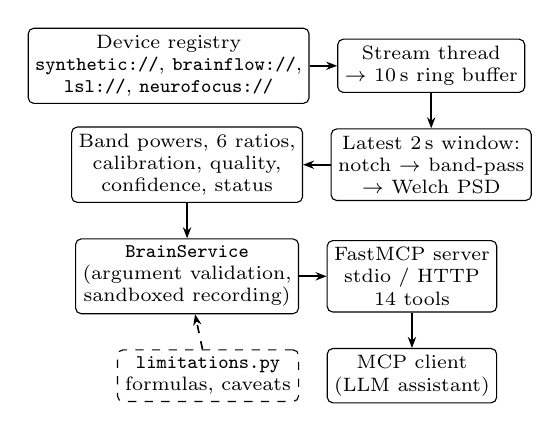
\begin{tikzpicture}[
  box/.style={draw,rounded corners=2pt,align=center,font=\scriptsize,
              minimum height=0.62cm,inner sep=2.5pt},
  arr/.style={-{Stealth[length=4pt]},semithick}]
\node[box,minimum width=2.3cm] (dev) {Device registry\\\texttt{synthetic://}, \texttt{brainflow://},\\\texttt{lsl://}, \texttt{neurofocus://}};
\node[box,right=0.35cm of dev,minimum width=2.1cm] (buf) {Stream thread\\$\rightarrow$ 10\,s ring buffer};
\node[box,below=0.45cm of buf,minimum width=2.1cm] (dsp) {Latest 2\,s window:\\notch $\rightarrow$ band-pass\\$\rightarrow$ Welch PSD};
\node[box,left=0.35cm of dsp,minimum width=2.3cm] (met) {Band powers, 6 ratios,\\calibration, quality,\\confidence, status};
\node[box,below=0.45cm of met,minimum width=2.3cm] (svc) {\texttt{BrainService}\\(argument validation,\\sandboxed recording)};
\node[box,right=0.35cm of svc,minimum width=2.1cm] (mcp) {FastMCP server\\stdio / HTTP\\14 tools};
\node[box,below=0.45cm of mcp,minimum width=2.1cm] (llm) {MCP client\\(LLM assistant)};
\node[box,left=0.35cm of llm,minimum width=2.3cm,dashed] (lim) {\texttt{limitations.py}\\formulas, caveats};
\draw[arr] (dev) -- (buf); \draw[arr] (buf) -- (dsp); \draw[arr] (dsp) -- (met);
\draw[arr] (met) -- (svc); \draw[arr] (svc) -- (mcp); \draw[arr] (mcp) -- (llm);
\draw[arr,dashed] (lim) -- (svc);
\end{tikzpicture}
\caption{Data flow. The model receives only computed scalars, each with quality
and confidence fields and the text of the pipeline's limitations.}
\label{fig:arch}
\end{figure}

\paragraph{Acquisition.} Every backend implements a five-method
\texttt{Device} interface and registers a URI scheme. Supported sources are a
synthetic generator, BrainFlow boards (OpenBCI, Muse and others), LSL streams,
a generic serial device, the NeuroFocus dry-electrode ear-EEG prototype over USB
serial and Bluetooth LE, and playback of recorded files. A single daemon thread
drains the device into a 10\,s multi-channel ring buffer (Figure~\ref{fig:arch}).

\paragraph{Signal processing.} On request, the pipeline takes the latest 2\,s
window. It applies a 60\,Hz IIR notch ($Q=30$) \emph{before} a 1--45\,Hz
fourth-order Butterworth band-pass, both zero-phase (\texttt{filtfilt}), then
estimates the power spectral density with Welch's method~\citep{welch1967}
(${\approx}1$\,s segments, 50\% overlap) using SciPy~\citep{virtanen2020} and
NumPy~\citep{harris2020}. Band power is the integral of the PSD over
$\delta$ (1--4\,Hz), $\theta$ (4--8), $\alpha$ (8--13), $\beta$ (13--30) and
$\gamma$ (30--45\,Hz), averaged over channels, with rectangular integration when
a narrow band covers a single frequency bin.

\paragraph{Metrics.} Six ratios are computed from $\theta$, $\alpha$ and
$\beta$ only (Table~\ref{tab:metrics}). Delta and gamma are reported but excluded
from every metric because, on consumer hardware over short windows, they are
dominated by drift and muscle activity. Uncalibrated, each ratio is mapped to
$[0,1]$ by a logistic centred at a neutral value (1.0 for unbounded ratios, 0.5
for the two bounded ones). A 20\,s calibration replaces this with a per-user
$z$-score baseline.

\begin{table}[t]
\centering\small
\caption{Metrics exposed to the model. All are heuristic proxies.}
\label{tab:metrics}
\begin{tabular}{@{}lll@{}}
\toprule
Metric & Formula & Basis \\
\midrule
focus      & $\beta/(\alpha+\theta)$        & Pope et al.~\citep{pope1995} \\
attention  & $\beta/\theta$                 & inverse TBR~\citep{monastra1999,arns2013} \\
fatigue    & $(\theta+\alpha)/\beta$        & Eoh et al.~\citep{eoh2005} \\
engagement & $\beta/\alpha$                 & arousal ratio \\
calm       & $\alpha/(\alpha+\beta)$        & alpha relaxation~\citep{barry2007} \\
meditation & $\alpha/(\alpha+\beta+\theta)$ & relative alpha~\citep{berger1929} \\
\bottomrule
\end{tabular}
\end{table}

\paragraph{Quality and confidence.} Each window is checked for flatline
(variance ${<}10^{-3}\,\mu\mathrm{V}^2$), railing (mean peak-to-peak
${>}2000\,\mu$V), probable EMG (${>}400\,\mu$V peak-to-peak) and blinks
(${>}150\,\mu$V deviation on the first channel). Flatline, railing or ``poor''
quality mark the reading \texttt{unreliable}. Confidence is the product of the
quality score, a calibration factor (1.0 calibrated, 0.6 not) and window fill,
and is capped at 0.1 when unreliable.

\paragraph{Honesty layer.} One module holds the analysis parameters, a list of
seven limitations (for example, Welch averaging makes the pipeline blind to
event-related potentials and spindles), and a one-line disclaimer. Every
\texttt{get\_brain\_state} reply carries the disclaimer;
\texttt{get\_metric\_definitions} and \texttt{get\_pipeline\_limitations} return
the full text; and the \texttt{interpret\_brain\_state} prompt instructs the
model to state those limits.

\paragraph{MCP interface and security.} The server uses the official MCP Python
SDK over stdio (local) or streamable HTTP. It exposes 14 tools (device listing
and connection, brain state, band powers, signal quality, definitions,
limitations, calibration, event marking, summary, recording, neurofeedback), the
resources \texttt{brain://state} and \texttt{brain://device}, and one prompt.
Because tool arguments come from a model that may be steered by untrusted
content, all arguments are validated and bounded, recordings are confined to a
sandbox directory with path-traversal and symlink checks, device schemes that
grant file or port access (\texttt{playback://}, \texttt{serial://}) are refused
over MCP, HTTP transports support bearer-token authentication, and loopback
binds enable DNS-rebinding protection.

\paragraph{Engineering.} The package supports Python 3.10--3.14, has 149
hardware-free tests run in CI, and is distributed on PyPI and as an \texttt{npx}
launcher on npm. Documentation is at
\url{https://enkhbold470.github.io/bci-mcp/}.

\section{Evaluation}\label{sec:eval}

All experiments run the released pipeline code without modification. Scripts are
in \texttt{paper/benchmarks/} and their JSON outputs in \texttt{paper/results/};
timings were measured on an Apple M5 Pro laptop (Python 3.12).

\subsection{Implementation check on synthetic ground truth}
The synthetic device mixes 10\,Hz alpha, 20\,Hz beta and 6\,Hz theta sinusoids
with Gaussian noise; its \texttt{focus} parameter trades alpha amplitude for beta
amplitude. We swept the parameter from 0 to 1 in eleven steps with 50 windows
each (uncalibrated). All six metrics were monotonic in the parameter in the
expected direction (Spearman $\rho = +0.996$ for focus, attention and
engagement; $-0.996$ for calm, fatigue and meditation). Scaled \emph{focus} rose
from 0.27 to 0.99 and \emph{calm} fell from 0.92 to 0.10. This verifies the
implementation, not the physiology.

\subsection{Real EEG: the eyes-closed alpha increase}
Closing the eyes increases posterior alpha power~\citep{berger1929,barry2007},
so a correct alpha-based pipeline must detect it. We used the PhysioNet EEG
Motor Movement/Imagery Dataset~\citep{schalk2004,goldberger2000}: for each of
109 subjects, run 1 is a one-minute eyes-open baseline and run 2 a one-minute
eyes-closed baseline (64 channels, 160\,Hz). The method was fixed before looking
at results: take O1, Oz and O2; split each run into non-overlapping 2\,s windows
(30 per run, 6{,}540 in total); run the unmodified, uncalibrated pipeline on
each; and average per subject. The primary outcome was \emph{calm}.

\begin{figure}[t]
\centering
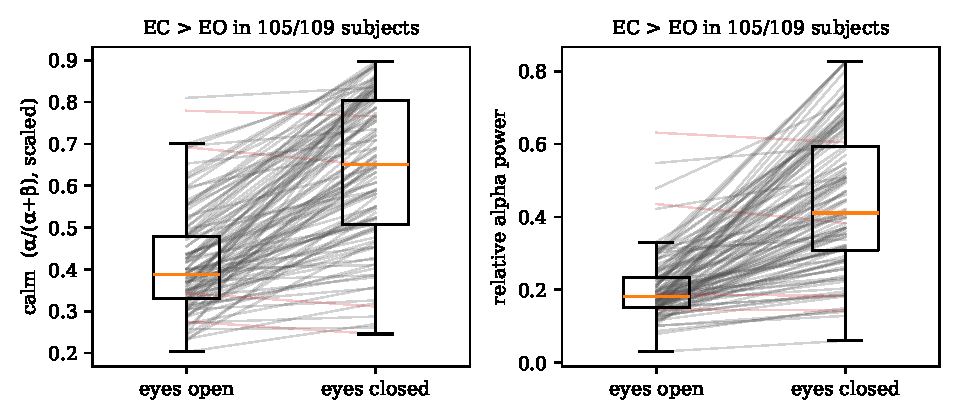
\includegraphics[width=\columnwidth]{../figures/eyes_closed.pdf}
\caption{Per-subject means, eyes open vs.\ closed (109 subjects). Grey lines
rise, red lines fall.}
\label{fig:ec}
\end{figure}

\begin{table}[t]
\centering\small
\caption{Eyes closed (EC) vs.\ eyes open (EO), 109 subjects. Medians of
per-subject means; Wilcoxon signed-rank; $r$ = matched-pairs rank-biserial;
AUC pools all windows.}
\label{tab:ec}
\begin{tabular}{@{}lccccc@{}}
\toprule
Outcome & EO & EC & EC$>$EO & $r$ & AUC \\
\midrule
calm (primary)  & 0.39 & 0.65 & 105/109 & $+0.99$ & 0.78 \\
meditation      & 0.25 & 0.53 & 106/109 & $+0.99$ & 0.80 \\
relative alpha  & 0.18 & 0.41 & 105/109 & $+0.99$ & 0.81 \\
focus           & 0.43 & 0.36 & 15/109  & $-0.85$ & 0.28 \\
\bottomrule
\end{tabular}
\end{table}

\emph{Calm} was higher with eyes closed in 105 of 109 subjects (median
difference $+0.21$, bootstrap 95\% CI $[0.17, 0.27]$; Wilcoxon $W = 33$,
$p = 3.2\times10^{-19}$), as were meditation and relative alpha
(Table~\ref{tab:ec}, Figure~\ref{fig:ec}). \emph{Focus}, whose denominator
contains alpha, fell as expected. Within subjects, a single threshold on
\emph{calm} separated eyes-closed from eyes-open windows with a median AUC of
0.87 (IQR 0.72--0.97). Pooled across subjects without calibration, the AUC was
0.78, which illustrates why per-user calibration exists. No window was marked
unreliable.

This is a check that the pipeline recovers a large, well-established effect, not
evidence that \emph{calm} measures calmness. The data are gel-electrode research
recordings, not consumer headsets.

\subsection{Artifact flagging}
We injected artifacts of known amplitude into clean synthetic windows (4
channels at 256\,Hz; 300 trials per cell). No clean window was flagged (0/300).
Blinks (a 200\,ms Gaussian on the first two channels) were flagged in 0\% of
trials at 100\,$\mu$V, 68\% at 150\,$\mu$V and 100\% from 200\,$\mu$V. Band-limited
30--100\,Hz noise standing in for EMG was missed at 50\,$\mu$V RMS and flagged
from 75\,$\mu$V RMS. Square-wave railing was marked unreliable from $\pm1000\,\mu$V,
and constant-offset flatlines in every trial.

Real data exposed a weakness. On the PhysioNet occipital windows, the blink
detector fired on 22.6\% of eyes-open and 39.5\% of eyes-closed windows. People do not
blink normally with their eyes closed, and occipital sites are far from the eyes,
so these flags are almost certainly false positives, triggered by large alpha. The detector is a pure
amplitude threshold on whichever channel is first, with no notion of montage or
waveform. A blink flag lowers neither status nor confidence, so the metrics above
are unaffected, but the flag itself misinforms the model. Montage-aware,
waveform-based blink detection is future work.

\subsection{Latency}
The per-window computation (filters, Welch, metrics, quality) had a median cost
of 0.35\,ms for 4 channels at 256\,Hz, 0.42\,ms for 8 channels at 250\,Hz and
0.94\,ms for 64 channels at 160\,Hz (2{,}000 repetitions each). End to end, we
launched \texttt{bci-mcp serve} as a subprocess and drove it with the official
MCP Python client over stdio, as a desktop assistant would. Cold start to a
completed \texttt{initialize} handshake took a median of 562\,ms (10 runs). After
\texttt{connect}, the first reading was available 387\,ms later (the buffer needs
0.5\,s of data). A \texttt{get\_brain\_state} call then had a median round trip
of 1.30\,ms (p95 2.34, p99 3.16\,ms; 500 calls; median reply 1.2\,kB). The
pipeline therefore adds negligible latency compared with LLM inference. Readings
describe the preceding 2\,s, and acquisition adds a device-dependent delay (for
example 125\,ms per chunk for the synthetic device), which we did not measure on
physical hardware.

\section{Limitations and ethical considerations}

The metrics are band-power ratios with literature precedent, not validated
measures of focus, calm or fatigue, and the tool must not be used for medical or
diagnostic purposes. The real-data evaluation covers one effect in one dataset of
research-grade recordings. It does not establish performance on dry-electrode
consumer devices, in motion, or for the attention and fatigue indices. Latency
was measured with synthetic acquisition on one machine. Welch averaging makes
the pipeline blind to transient events, and artifacts are flagged, not removed.

Neural data is sensitive. BCI-MCP runs locally by default and sends nothing
anywhere unless the user connects it to a cloud-hosted assistant, at which point
the computed metrics (not raw EEG) leave the machine with each tool call. Users
should understand that before connecting. The larger risk is interpretive: an
assistant may narrate a heuristic number as a fact about a person's mind. The
honesty layer reduces that risk, but whether models actually respect confidence
and limitation fields is untested and is the most important open question for
this kind of system.

\section{Availability}
Source (MIT): \url{https://github.com/enkhbold470/bci-mcp}. Install with
\texttt{pip install bci-mcp} or run \texttt{npx -y bci-mcp}. The evaluation is
reproduced by the scripts in \texttt{paper/benchmarks/}; the PhysioNet data is
freely downloadable.

\section*{AI usage disclosure}
Much of the June 2026 rewrite of BCI-MCP was written with AI coding assistants
(Claude Code, Cursor) working from design documents kept in the repository; the
author directed the design, integrated the NeuroFocus hardware protocol, reviewed
and tested the changes, and is responsible for the code. The benchmark scripts
and a first draft of this manuscript were also prepared with an AI assistant
(Claude). The author checked every number against the benchmark outputs and every
reference against its DOI record, and takes full responsibility for the content.

\section*{Acknowledgments}
We thank the creators of the EEG Motor Movement/Imagery Dataset and PhysioNet for
making the data public.

\small
\bibliographystyle{plainnat}
\bibliography{../paper}

\end{document}
